\documentclass[11pt]{article}

\usepackage[T1]{fontenc}
\usepackage[utf8]{inputenc}
\usepackage{lmodern}
\usepackage[a4paper,margin=1in]{geometry}
\usepackage{amsmath,amssymb,amsthm,mathtools}
\usepackage{enumitem}
\usepackage{booktabs}
\usepackage{xcolor}
\usepackage{tikz}
\usepackage{tcolorbox}
\usepackage{hyperref}
\usetikzlibrary{arrows.meta,positioning,calc,backgrounds,fit}
\tcbuselibrary{skins,breakable}

\hypersetup{colorlinks=true,linkcolor=blue!70!black,citecolor=blue!70!black,urlcolor=blue!70!black}

% ── Drawing styles ────────────────────────────────────────────────────────────
\tikzset{
  orig/.style   ={circle,draw,thick,minimum size=8mm,inner sep=0pt,font=\small},
  slot/.style   ={circle,draw,minimum size=8.5mm,inner sep=0pt,font=\scriptsize},
  c1/.style     ={fill=red!28},
  c2/.style     ={fill=blue!22},
  c3/.style     ={fill=yellow!55},
  chosen/.style ={line width=1.1pt,draw=green!55!black},
  choiceedge/.style  ={gray,thick},
  conflictedge/.style={red!65!black,thick},
  atom/.style   ={circle,draw,fill=black,minimum size=2.4mm,inner sep=0pt},
}
\newcommand{\colorlegend}{%
  \tikz[baseline=-0.6ex]{\node[slot,c1,minimum size=5mm]{};} color~1\quad
  \tikz[baseline=-0.6ex]{\node[slot,c2,minimum size=5mm]{};} color~2\quad
  \tikz[baseline=-0.6ex]{\node[slot,c3,minimum size=5mm]{};} color~3}

\title{\textbf{Worked Examples: Compiling Graph Coloring to a\\ Unit-Disk Independent-Set Problem}\\[0.4em]
\large A step-by-step companion, nothing skipped}
\author{Teaching Supplement}
\date{\today}

\begin{document}
\maketitle

\begin{abstract}
This companion document walks, in full detail, through the transformation that
turns a graph-coloring question into the maximum-independent-set (MIS) problem a
neutral-atom machine actually solves. It is written for a reader meeting the
construction for the first time: every vertex, every edge, and every reasoning
step is shown. We treat five graphs of increasing interest --- a single edge, a
path, a triangle, a square, and a pentagon --- and for the smallest one we also
carry it all the way onto a unit-disk geometry and solve it by hand. The
underlying reduction and pipeline are those of the main
paper~\cite{Karp1972,Pichler2018,Nguyen2023}.
\end{abstract}

\tableofcontents

% =============================================================================
\section{The rules of the game}
% =============================================================================

We want to know whether a graph $G=(V,E)$ can be properly colored with $k$ colors:
can we assign each vertex one of $k$ colors so that \emph{no edge joins two
vertices of the same color}? The hardware cannot answer this directly --- it only
finds large \emph{independent sets} (sets of mutually non-adjacent vertices) of a
\emph{unit-disk graph}. So we translate. The translation has two stages.

\begin{tcolorbox}[colback=blue!4,colframe=blue!55!black,title=\textbf{Stage 1
  --- the color-choice graph $G'$ (exact, the heart of everything)},breakable]
Start from $G=(V,E)$ with $n=|V|$ vertices and $m=|E|$ edges, and a palette of
$k$ colors.
\begin{enumerate}[leftmargin=1.6em,itemsep=2pt]
  \item \textbf{Make $k$ copies of every vertex.} The new vertex set is
        \[ V' = V\times\{1,\dots,k\} = \{(v,i) : v\in V,\ i\in\{1,\dots,k\}\}. \]
        Read $(v,i)$ as the statement ``\emph{vertex $v$ takes color $i$}.''
        There are $|V'| = n\,k$ slots.
  \item \textbf{Choice edges (one color per vertex).} For each original vertex
        $v$, join all of its $k$ slots into a clique:
        \[ \{(v,i),(v,j)\}\ \text{for all } i<j. \]
        Because an independent set may contain \emph{at most one} vertex of a
        clique, this forces ``$v$ gets \emph{at most} one color.'' This adds
        $\binom{k}{2}$ edges per vertex.
  \item \textbf{Conflict edges (adjacent vertices differ).} For each original
        edge $\{u,v\}\in E$ and each color $i$, join the two slots of that color:
        \[ \{(u,i),(v,i)\}. \]
        This forbids $u$ and $v$ from \emph{both} taking color $i$. This adds
        $k$ edges per original edge.
\end{enumerate}
In total $|E'| = n\binom{k}{2} + m\,k$.

\medskip
\textbf{The payoff.} A set $S\subseteq V'$ is independent and has size $n$
\emph{exactly when} it picks one slot per vertex with no conflict --- i.e.\
\emph{exactly when} it is a proper $k$-coloring. Hence
\[
   \boxed{\ \alpha(G') = n \iff G \text{ is } k\text{-colorable},\ }
\]
where $\alpha$ is the size of the largest independent set, and $\alpha(G')\le n$
always (at most one slot per vertex).
\end{tcolorbox}

\begin{tcolorbox}[colback=green!4,colframe=green!45!black,title=\textbf{Stage 2
  --- realize $G'$ as a unit-disk graph the machine can run}]
$G'$ is still an abstract graph. Stage 2 \emph{places} its vertices (now ``atoms'')
as points in the plane and picks a radius $r$ so that two atoms are adjacent
precisely when they are within distance $r$. When $G'$ is not directly a unit-disk
graph, small \emph{copy} and \emph{crossing} gadgets reproduce the required
adjacencies~\cite{Pichler2018,Nguyen2023}. The machine then finds the
maximum-weight independent set of this geometry, and we \emph{decode}: read off,
for each original vertex, which color-slot was chosen. We carry this stage out by
hand for the single-edge example in Section~\ref{sec:geometry}.
\end{tcolorbox}

\paragraph{How to read the diagrams.} For each graph we draw three things:
the original graph $G$; the color-choice graph $G'$ as a \emph{grid}, with one
\textbf{column per original vertex} and one \textbf{row per color}, so the slot
$(v,i)$ sits in column $v$, row $i$; and finally $G$ again, colored by the answer
we decode. In the grid, \textcolor{gray}{\textbf{gray}} edges are choice edges
(vertical, within a column) and \textcolor{red!65!black}{\textbf{red}} edges are
conflict edges (within a row). A \textcolor{green!55!black}{\textbf{green ring}}
marks the chosen independent set. Color key: \colorlegend.

% =============================================================================
\section{Example 1 --- a single edge \texorpdfstring{$K_2$}{K2}}
% =============================================================================

\textbf{The graph.} $G$ has two vertices $u,v$ and one edge. Clearly two colors
suffice, and one will not (the two endpoints must differ). Let us watch the
machinery confirm $k=2$.

\begin{center}
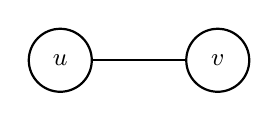
\begin{tikzpicture}
  \node[orig] (u) at (0,0) {$u$};
  \node[orig] (v) at (2,0) {$v$};
  \draw[thick] (u)--(v);
\end{tikzpicture}
\end{center}

\noindent $n=2$, $m=1$, $k=2$.

\paragraph{Step 1 --- the slots.} Two vertices $\times$ two colors give
$|V'|=nk=4$ slots:
\[ (u,1),\ (u,2),\ (v,1),\ (v,2). \]

\paragraph{Step 2 --- choice edges.} One clique per vertex; with $k=2$ a clique is
a single edge ($\binom{2}{2}=1$ edge each):
\[ \{(u,1),(u,2)\},\qquad \{(v,1),(v,2)\}. \]

\paragraph{Step 3 --- conflict edges.} The single edge $\{u,v\}$ contributes one
conflict edge per color:
\[ \text{color 1:}\ \{(u,1),(v,1)\}, \qquad \text{color 2:}\ \{(u,2),(v,2)\}. \]

\paragraph{Step 4 --- tally.} $|V'|=4$ and
$|E'| = n\binom{k}{2}+mk = 2\cdot 1 + 1\cdot 2 = 4$. Here is $G'$:

\begin{center}
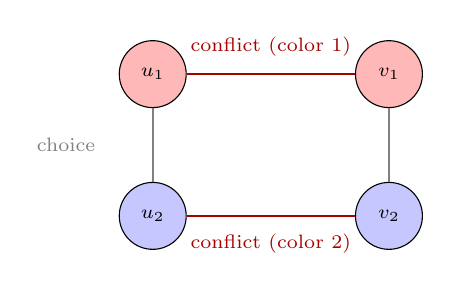
\begin{tikzpicture}
  \node[slot,c1] (u1) at (0,0)    {$u_1$};
  \node[slot,c2] (u2) at (0,-1.8) {$u_2$};
  \node[slot,c1] (v1) at (3,0)    {$v_1$};
  \node[slot,c2] (v2) at (3,-1.8) {$v_2$};
  \draw[choiceedge] (u1)--(u2);
  \draw[choiceedge] (v1)--(v2);
  \draw[conflictedge] (u1)--(v1);
  \draw[conflictedge] (u2)--(v2);
  \node[font=\scriptsize,gray] at (-1.1,-0.9) {choice};
  \node[font=\scriptsize,red!65!black] at (1.5,0.35) {conflict (color 1)};
  \node[font=\scriptsize,red!65!black] at (1.5,-2.15) {conflict (color 2)};
\end{tikzpicture}
\end{center}

Notice $G'$ is a $4$-cycle $u_1-u_2-v_2-v_1-u_1$.

\paragraph{Step 5 --- find the largest independent set.} We may take at most one
slot from each column (the choice edge forbids both). Try one per column:
choosing $(u,1)$ rules out $(v,1)$ (conflict, color~1), leaving $(v,2)$. Check the
pair $S=\{(u,1),(v,2)\}$: $(u,1)$'s neighbors are $(u,2)$ and $(v,1)$ --- neither is
$(v,2)$ --- so $S$ is independent, and $|S|=2=n$.

\begin{center}
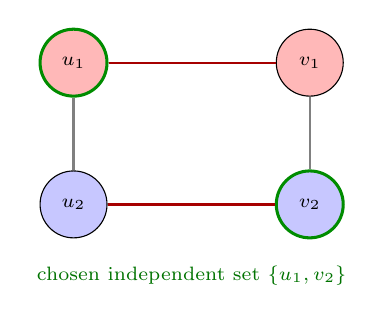
\begin{tikzpicture}
  \node[slot,c1,chosen] (u1) at (0,0)    {$u_1$};
  \node[slot,c2]        (u2) at (0,-1.8) {$u_2$};
  \node[slot,c1]        (v1) at (3,0)    {$v_1$};
  \node[slot,c2,chosen] (v2) at (3,-1.8) {$v_2$};
  \draw[choiceedge] (u1)--(u2);
  \draw[choiceedge] (v1)--(v2);
  \draw[conflictedge] (u1)--(v1);
  \draw[conflictedge] (u2)--(v2);
  \node[font=\scriptsize,green!45!black] at (1.5,-2.7) {chosen independent set $\{u_1,v_2\}$};
\end{tikzpicture}
\end{center}

\paragraph{Step 6 --- the verdict.} $\alpha(G')=2=n$, so by the boxed rule $G$
\emph{is} $2$-colorable.

\paragraph{Step 7 --- decode.} The chosen slots say $u\mapsto$ color~1,
$v\mapsto$ color~2. Restoring this onto $G$:

\begin{center}
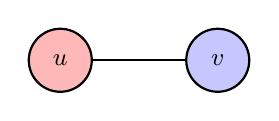
\begin{tikzpicture}
  \node[orig,c1] (u) at (0,0) {$u$};
  \node[orig,c2] (v) at (2,0) {$v$};
  \draw[thick] (u)--(v);
\end{tikzpicture}
\end{center}
A proper $2$-coloring, exactly as expected.

% =============================================================================
\section{Example 2 --- a path \texorpdfstring{$P_3$}{P3}}
% =============================================================================

\textbf{The graph.} Three vertices in a line, $a-b-c$. It is bipartite, so two
colors suffice. $n=3$, $m=2$, $k=2$.

\begin{center}
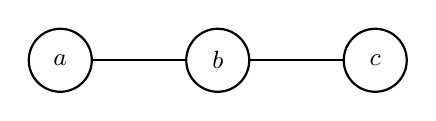
\begin{tikzpicture}
  \node[orig](a) at (0,0){$a$}; \node[orig](b) at (2,0){$b$}; \node[orig](c) at (4,0){$c$};
  \draw[thick](a)--(b)--(c);
\end{tikzpicture}
\end{center}

\paragraph{Step 1 --- slots.} $|V'|=nk=6$: $(a,1),(a,2),(b,1),(b,2),(c,1),(c,2)$.

\paragraph{Step 2 --- choice edges.} One per column:
$\{(a,1),(a,2)\},\ \{(b,1),(b,2)\},\ \{(c,1),(c,2)\}$.

\paragraph{Step 3 --- conflict edges.} Two original edges $\{a,b\}$ and
$\{b,c\}$, each duplicated over the two colors:
\[
\text{from } ab:\ \{(a,1),(b,1)\},\{(a,2),(b,2)\};\qquad
\text{from } bc:\ \{(b,1),(c,1)\},\{(b,2),(c,2)\}.
\]
There is \emph{no} conflict edge between columns $a$ and $c$, because $a$ and $c$
are \emph{not} adjacent in $G$ --- a point we exploit in a moment.

\paragraph{Step 4 --- tally.} $|E'| = 3\cdot 1 + 2\cdot 2 = 7$. Here is $G'$:

\begin{center}
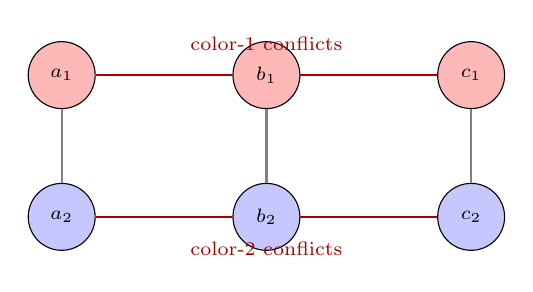
\begin{tikzpicture}
  \foreach \x/\name in {0/a,2.6/b,5.2/c}{
     \node[slot,c1] (\name1) at (\x,0)    {$\name_1$};
     \node[slot,c2] (\name2) at (\x,-1.8) {$\name_2$};
     \draw[choiceedge] (\name1)--(\name2);
  }
  \draw[conflictedge] (a1)--(b1); \draw[conflictedge] (b1)--(c1);
  \draw[conflictedge] (a2)--(b2); \draw[conflictedge] (b2)--(c2);
  \node[font=\scriptsize,red!65!black] at (2.6,0.4) {color-1 conflicts};
  \node[font=\scriptsize,red!65!black] at (2.6,-2.2) {color-2 conflicts};
\end{tikzpicture}
\end{center}

\paragraph{Step 5 --- largest independent set.} The standard proper coloring is
$a=1,\ b=2,\ c=1$. The matching slots are $S=\{(a,1),(b,2),(c,1)\}$. Check:
$(a,1)$ touches only $(a,2),(b,1)$; $(b,2)$ touches only $(b,1),(a,2),(c,2)$;
$(c,1)$ touches only $(c,2),(b,1)$. None of these hit another member of $S$ ---
in particular $(a,1)$ and $(c,1)$ share row~1 but are \emph{not} joined, since
$a,c$ are non-adjacent. So $S$ is independent and $|S|=3=n$.

\begin{center}
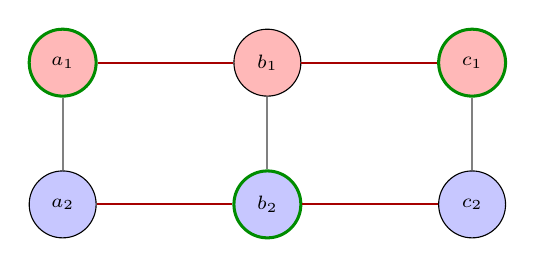
\begin{tikzpicture}
  \node[slot,c1,chosen] (a1) at (0,0){$a_1$};    \node[slot,c2] (a2) at (0,-1.8){$a_2$};
  \node[slot,c1]        (b1) at (2.6,0){$b_1$};  \node[slot,c2,chosen] (b2) at (2.6,-1.8){$b_2$};
  \node[slot,c1,chosen] (c1) at (5.2,0){$c_1$};  \node[slot,c2] (c2) at (5.2,-1.8){$c_2$};
  \foreach \n in {a,b,c}{\draw[choiceedge] (\n1)--(\n2);}
  \draw[conflictedge] (a1)--(b1); \draw[conflictedge] (b1)--(c1);
  \draw[conflictedge] (a2)--(b2); \draw[conflictedge] (b2)--(c2);
\end{tikzpicture}
\end{center}

\paragraph{Steps 6--7 --- verdict and decode.} $\alpha(G')=3=n$: $G$ is
$2$-colorable, with $a=1,\ b=2,\ c=1$.

\begin{center}
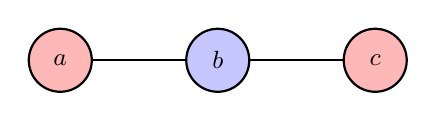
\begin{tikzpicture}
  \node[orig,c1](a) at (0,0){$a$}; \node[orig,c2](b) at (2,0){$b$}; \node[orig,c1](c) at (4,0){$c$};
  \draw[thick](a)--(b)--(c);
\end{tikzpicture}
\end{center}

% =============================================================================
\section{Example 3 --- a triangle \texorpdfstring{$K_3$}{K3}: when $k$ is too small}
% =============================================================================

\textbf{The graph.} Three mutually adjacent vertices $a,b,c$. Every pair is an
edge, so all three must receive \emph{different} colors: $\chi(K_3)=3$. We
deliberately first \emph{try $k=2$ and watch it fail}, then succeed with $k=3$.
$n=3$, $m=3$.

\begin{center}
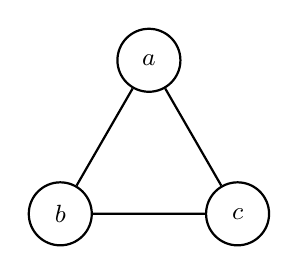
\begin{tikzpicture}
  \node[orig](a) at (90:1.3){$a$}; \node[orig](b) at (210:1.3){$b$}; \node[orig](c) at (330:1.3){$c$};
  \draw[thick](a)--(b)--(c)--(a);
\end{tikzpicture}
\end{center}

\subsection{Attempt with $k=2$ (must fail)}

\paragraph{Steps 1--3.} Slots $\{(a,i),(b,i),(c,i):i=1,2\}$, $|V'|=6$. Choice
edges per column as usual. Now \emph{every} original edge is present, so for each
color $i$ the three slots $(a,i),(b,i),(c,i)$ are pairwise joined --- each row is
itself a triangle:
\[
\text{color 1:}\ \{(a,1),(b,1)\},\{(b,1),(c,1)\},\{(a,1),(c,1)\};\quad
\text{color 2: the same with subscript } 2.
\]
$|E'| = 3\cdot 1 + 3\cdot 2 = 9$.

\begin{center}
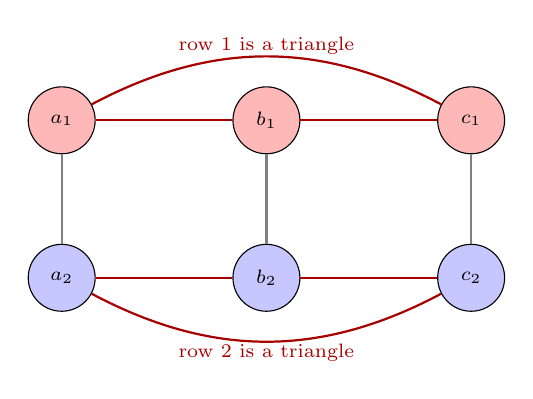
\begin{tikzpicture}
  \foreach \x/\name in {0/a,2.6/b,5.2/c}{
     \node[slot,c1] (\name1) at (\x,0){$\name_1$};
     \node[slot,c2] (\name2) at (\x,-2.0){$\name_2$};
     \draw[choiceedge] (\name1)--(\name2);
  }
  % row1 triangle
  \draw[conflictedge] (a1)--(b1)--(c1);
  \draw[conflictedge] (a1) to[bend left=28] (c1);
  % row2 triangle
  \draw[conflictedge] (a2)--(b2)--(c2);
  \draw[conflictedge] (a2) to[bend right=28] (c2);
  \node[font=\scriptsize,red!65!black] at (2.6,0.95) {row 1 is a triangle};
  \node[font=\scriptsize,red!65!black] at (2.6,-2.95){row 2 is a triangle};
\end{tikzpicture}
\end{center}

\paragraph{Step 5 --- why size $3$ is impossible.} An independent set takes at
most one slot per column, so at most $3$ slots, one in each of columns $a,b,c$.
Those three live in only \emph{two} rows, so by the pigeonhole principle two of
them share a row. But within a row \emph{every} pair is a conflict edge --- so
those two are adjacent, contradicting independence. Hence no independent set of
size $3$ exists. The best we can do is size $2$, e.g.\ $\{(a,1),(b,2)\}$:

\begin{center}
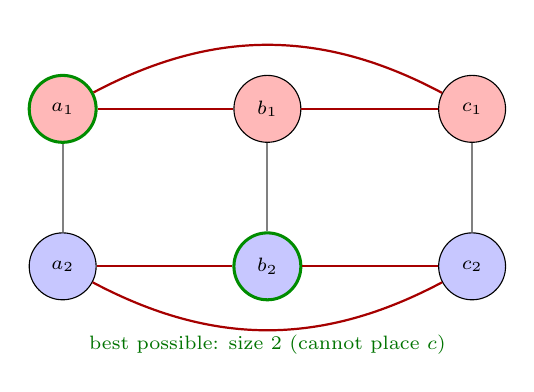
\begin{tikzpicture}
  \node[slot,c1,chosen](a1) at (0,0){$a_1$};   \node[slot,c2](a2) at (0,-2.0){$a_2$};
  \node[slot,c1](b1) at (2.6,0){$b_1$};        \node[slot,c2,chosen](b2) at (2.6,-2.0){$b_2$};
  \node[slot,c1](c1) at (5.2,0){$c_1$};        \node[slot,c2](c2) at (5.2,-2.0){$c_2$};
  \foreach \n in {a,b,c}{\draw[choiceedge](\n1)--(\n2);}
  \draw[conflictedge](a1)--(b1)--(c1); \draw[conflictedge](a1) to[bend left=28](c1);
  \draw[conflictedge](a2)--(b2)--(c2); \draw[conflictedge](a2) to[bend right=28](c2);
  \node[font=\scriptsize,green!45!black] at (2.6,-3.0){best possible: size $2$ (cannot place $c$)};
\end{tikzpicture}
\end{center}

\paragraph{Step 6 --- verdict.} $\alpha(G')=2<3=n$, so $G$ is \emph{not}
$2$-colorable. The reduction reports failure honestly: there simply is no
size-$n$ independent set to find.

\subsection{Attempt with $k=3$ (succeeds)}

Now each vertex has three slots, $|V'|=nk=9$. Choice edges make each column a
triangle; conflict edges make each of the three rows a triangle.
$|E'| = 3\binom{3}{2} + 3\cdot 3 = 9 + 9 = 18$.

\begin{center}
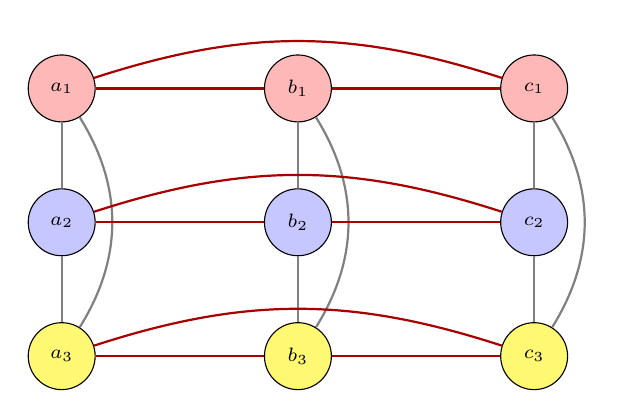
\begin{tikzpicture}[scale=1]
  \foreach \x/\name in {0/a,3/b,6/c}{
     \node[slot,c1] (\name1) at (\x,0){$\name_1$};
     \node[slot,c2] (\name2) at (\x,-1.7){$\name_2$};
     \node[slot,c3] (\name3) at (\x,-3.4){$\name_3$};
     % choice triangle within column
     \draw[choiceedge] (\name1)--(\name2)--(\name3);
     \draw[choiceedge] (\name1) to[bend left=32] (\name3);
  }
  \foreach \y in {1,2,3}{
     \draw[conflictedge] (a\y)--(b\y)--(c\y);
     \draw[conflictedge] (a\y) to[bend left=18] (c\y);
  }
\end{tikzpicture}
\end{center}

\paragraph{Step 5 --- a size-$3$ set now exists.} Put each vertex in a
\emph{different} row: $S=\{(a,1),(b,2),(c,3)\}$. Members lie in distinct columns
(no choice edge) \emph{and} distinct rows (conflict edges only ever join slots in
the \emph{same} row), so no edge joins any two of them. $S$ is independent and
$|S|=3=n$.

\begin{center}
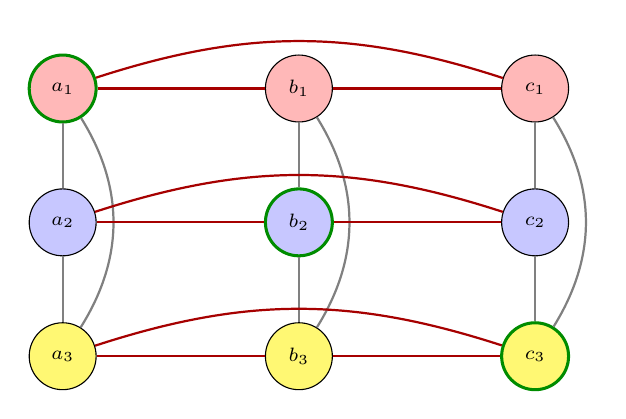
\begin{tikzpicture}
  \node[slot,c1,chosen](a1) at (0,0){$a_1$};  \node[slot,c2](a2) at (0,-1.7){$a_2$};  \node[slot,c3](a3) at (0,-3.4){$a_3$};
  \node[slot,c1](b1) at (3,0){$b_1$};         \node[slot,c2,chosen](b2) at (3,-1.7){$b_2$}; \node[slot,c3](b3) at (3,-3.4){$b_3$};
  \node[slot,c1](c1) at (6,0){$c_1$};         \node[slot,c2](c2) at (6,-1.7){$c_2$};  \node[slot,c3,chosen](c3) at (6,-3.4){$c_3$};
  \foreach \n in {a,b,c}{\draw[choiceedge](\n1)--(\n2)--(\n3); \draw[choiceedge](\n1) to[bend left=32](\n3);}
  \foreach \y in {1,2,3}{\draw[conflictedge](a\y)--(b\y)--(c\y); \draw[conflictedge](a\y) to[bend left=18](c\y);}
\end{tikzpicture}
\end{center}

\paragraph{Steps 6--7 --- verdict and decode.} $\alpha(G')=3=n$: $K_3$ is
$3$-colorable, decoded as $a=1,\ b=2,\ c=3$ --- three different colors, as it must
be.

\begin{center}
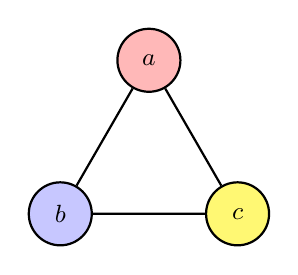
\begin{tikzpicture}
  \node[orig,c1](a) at (90:1.3){$a$}; \node[orig,c2](b) at (210:1.3){$b$}; \node[orig,c3](c) at (330:1.3){$c$};
  \draw[thick](a)--(b)--(c)--(a);
\end{tikzpicture}
\end{center}

\begin{tcolorbox}[colback=gray!6,colframe=gray!55,title=\textbf{Lesson}]
The same graph fails at $k=2$ and succeeds at $k=3$. To find the \emph{chromatic
number} we simply try increasing $k$ and report the first that yields
$\alpha(G')=n$. For $K_3$ that first success is $k=3$, so $\chi(K_3)=3$.
\end{tcolorbox}

% =============================================================================
\section{Example 4 --- a square \texorpdfstring{$C_4$}{C4} (even cycle)}
% =============================================================================

\textbf{The graph.} A $4$-cycle $a-b-c-d-a$. Even cycles are bipartite, so two
colors suffice. $n=4$, $m=4$, $k=2$.

\begin{center}
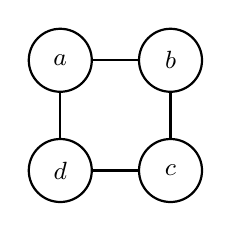
\begin{tikzpicture}
  \node[orig](a) at (0,1.4){$a$}; \node[orig](b) at (1.4,1.4){$b$};
  \node[orig](c) at (1.4,0){$c$};  \node[orig](d) at (0,0){$d$};
  \draw[thick](a)--(b)--(c)--(d)--(a);
\end{tikzpicture}
\end{center}

\paragraph{Steps 1--3.} $|V'|=8$. Choice edges per column. The four original
edges $ab,bc,cd,da$ each appear in both colors. So in each row the conflict edges
trace the same $4$-cycle on the columns: $a_i-b_i-c_i-d_i-a_i$. Crucially there is
\emph{no} edge between columns $a$ and $c$, nor between $b$ and $d$ (those pairs
are non-adjacent in $G$). $|E'| = 4\cdot 1 + 4\cdot 2 = 12$.

\begin{center}
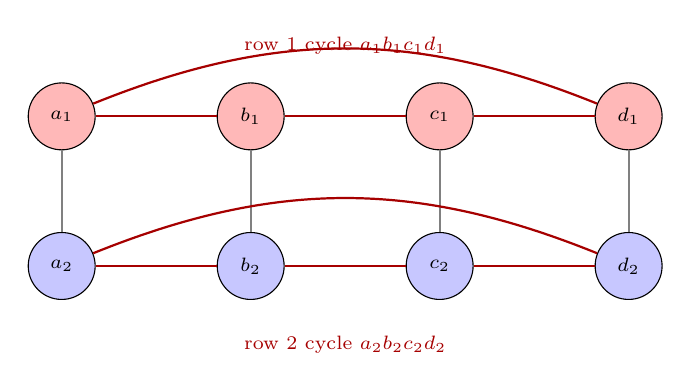
\begin{tikzpicture}
  \foreach \x/\name in {0/a,2.4/b,4.8/c,7.2/d}{
     \node[slot,c1] (\name1) at (\x,0){$\name_1$};
     \node[slot,c2] (\name2) at (\x,-1.9){$\name_2$};
     \draw[choiceedge] (\name1)--(\name2);
  }
  \foreach \y in {1,2}{
     \draw[conflictedge] (a\y)--(b\y)--(c\y)--(d\y);
     \draw[conflictedge] (a\y) to[bend left=22] (d\y); % wrap edge d-a
  }
  \node[font=\scriptsize,red!65!black] at (3.6,0.9){row 1 cycle $a_1 b_1 c_1 d_1$};
  \node[font=\scriptsize,red!65!black] at (3.6,-2.9){row 2 cycle $a_2 b_2 c_2 d_2$};
\end{tikzpicture}
\end{center}

\paragraph{Step 5 --- largest independent set.} The proper $2$-coloring alternates
around the square: $a=1,\ b=2,\ c=1,\ d=2$. The slots are
$S=\{(a,1),(b,2),(c,1),(d,2)\}$. The two row-$1$ members $(a,1),(c,1)$ are
\emph{not} adjacent (no $a$--$c$ edge), and likewise $(b,2),(d,2)$ are not
adjacent; across rows there are no conflicts. So $S$ is independent, $|S|=4=n$.

\begin{center}
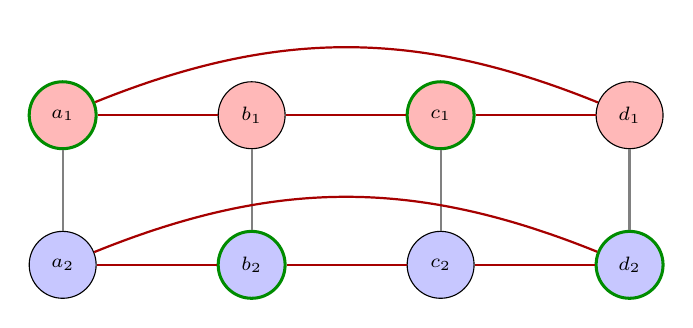
\begin{tikzpicture}
  \node[slot,c1,chosen](a1) at (0,0){$a_1$};   \node[slot,c2](a2) at (0,-1.9){$a_2$};
  \node[slot,c1](b1) at (2.4,0){$b_1$};        \node[slot,c2,chosen](b2) at (2.4,-1.9){$b_2$};
  \node[slot,c1,chosen](c1) at (4.8,0){$c_1$}; \node[slot,c2](c2) at (4.8,-1.9){$c_2$};
  \node[slot,c1](d1) at (7.2,0){$d_1$};        \node[slot,c2,chosen](d2) at (7.2,-1.9){$d_2$};
  \foreach \n in {a,b,c,d}{\draw[choiceedge](\n1)--(\n2);}
  \foreach \y in {1,2}{\draw[conflictedge](a\y)--(b\y)--(c\y)--(d\y); \draw[conflictedge](a\y) to[bend left=22](d\y);}
\end{tikzpicture}
\end{center}

\paragraph{Steps 6--7 --- verdict and decode.} $\alpha(G')=4=n$: $C_4$ is
$2$-colorable, $a=c=1$, $b=d=2$.

\begin{center}
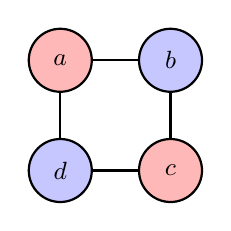
\begin{tikzpicture}
  \node[orig,c1](a) at (0,1.4){$a$}; \node[orig,c2](b) at (1.4,1.4){$b$};
  \node[orig,c1](c) at (1.4,0){$c$};  \node[orig,c2](d) at (0,0){$d$};
  \draw[thick](a)--(b)--(c)--(d)--(a);
\end{tikzpicture}
\end{center}

% =============================================================================
\section{Example 5 --- a pentagon \texorpdfstring{$C_5$}{C5} (odd cycle)}
% =============================================================================

\textbf{The graph.} A $5$-cycle $a-b-c-d-e-a$. Odd cycles are the smallest graphs
that are \emph{not} bipartite: two colors fail, three succeed, so $\chi(C_5)=3$.
Contrast this with the even cycle $C_4$ above --- the parity of the cycle is the
whole story. $n=5$, $m=5$.

\begin{center}
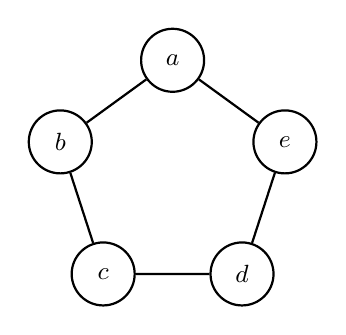
\begin{tikzpicture}
  \foreach \i/\name in {0/a,1/b,2/c,3/d,4/e}{
     \node[orig] (\name) at ({90+72*\i}:1.5){$\name$};
  }
  \draw[thick] (a)--(b)--(c)--(d)--(e)--(a);
\end{tikzpicture}
\end{center}

\subsection{Attempt with $k=2$ (must fail)}

\paragraph{Steps 1--3.} $|V'|=10$. Choice edge per column. Each of the five edges
$ab,bc,cd,de,ea$ appears in both rows, so each row is a $5$-cycle on the columns.
$|E'| = 5\cdot 1 + 5\cdot 2 = 15$.

\begin{center}
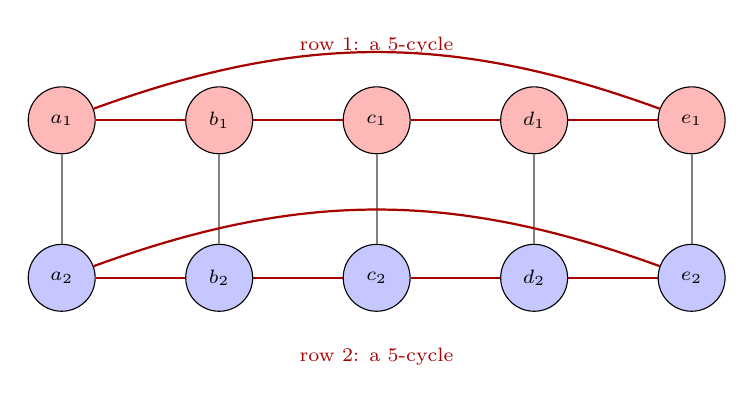
\begin{tikzpicture}
  \foreach \x/\name in {0/a,2/b,4/c,6/d,8/e}{
     \node[slot,c1] (\name1) at (\x,0){$\name_1$};
     \node[slot,c2] (\name2) at (\x,-2.0){$\name_2$};
     \draw[choiceedge] (\name1)--(\name2);
  }
  \foreach \y in {1,2}{
     \draw[conflictedge] (a\y)--(b\y)--(c\y)--(d\y)--(e\y);
     \draw[conflictedge] (a\y) to[bend left=20] (e\y); % wrap e-a
  }
  \node[font=\scriptsize,red!65!black] at (4,0.95){row 1: a 5-cycle};
  \node[font=\scriptsize,red!65!black] at (4,-3.0){row 2: a 5-cycle};
\end{tikzpicture}
\end{center}

\paragraph{Step 5 --- why it fails.} An independent set picks one slot from each
of the five columns, placing five members into only \emph{two} rows. Walk around
the cycle $a,b,c,d,e$: a $2$-coloring would have to alternate
$1,2,1,2,\dots$, but after five steps we return to $a$ with a clash --- an odd
cycle cannot be $2$-colored. Concretely, any one-per-column choice forces two
\emph{adjacent} vertices into the same row, and a same-row adjacent pair is a
conflict edge. So no independent set reaches size $5$; the best is size $4$, e.g.\
color $a,b,c,d$ as $1,2,1,2$ and leave $e$ out (both $e_1$ and $e_2$ clash --- $e_1$
with $a_1$, and $e_2$ with $d_2$):

\begin{center}
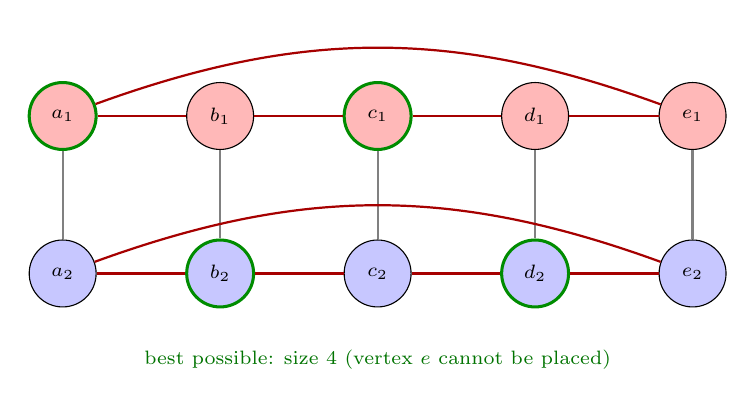
\begin{tikzpicture}
  \node[slot,c1,chosen](a1) at (0,0){$a_1$};  \node[slot,c2](a2) at (0,-2.0){$a_2$};
  \node[slot,c1](b1) at (2,0){$b_1$};         \node[slot,c2,chosen](b2) at (2,-2.0){$b_2$};
  \node[slot,c1,chosen](c1) at (4,0){$c_1$};  \node[slot,c2](c2) at (4,-2.0){$c_2$};
  \node[slot,c1](d1) at (6,0){$d_1$};         \node[slot,c2,chosen](d2) at (6,-2.0){$d_2$};
  \node[slot,c1](e1) at (8,0){$e_1$};         \node[slot,c2](e2) at (8,-2.0){$e_2$};
  \foreach \n in {a,b,c,d,e}{\draw[choiceedge](\n1)--(\n2);}
  \foreach \y in {1,2}{\draw[conflictedge](a\y)--(b\y)--(c\y)--(d\y)--(e\y); \draw[conflictedge](a\y) to[bend left=20](e\y);}
  \node[font=\scriptsize,green!45!black] at (4,-3.1){best possible: size $4$ (vertex $e$ cannot be placed)};
\end{tikzpicture}
\end{center}

\paragraph{Step 6 --- verdict.} $\alpha(G')=4<5=n$: $C_5$ is not $2$-colorable.

\subsection{Attempt with $k=3$ (succeeds)}

Add a third row. $|V'|=15$, $|E'| = 5\binom{3}{2} + 5\cdot 3 = 15 + 15 = 30$. A
proper $3$-coloring of the pentagon is $a=1,\ b=2,\ c=1,\ d=2,\ e=3$: the new third
color rescues the one vertex that the alternation could not place. The matching
independent set is $S=\{(a,1),(b,2),(c,1),(d,2),(e,3)\}$.

\begin{center}
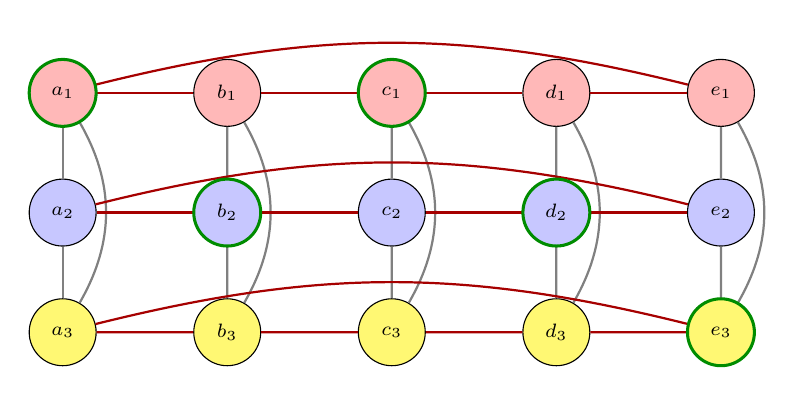
\begin{tikzpicture}[scale=0.95]
  \foreach \x/\name in {0/a,2.2/b,4.4/c,6.6/d,8.8/e}{
     \node[slot,c1] (\name1) at (\x,0){$\name_1$};
     \node[slot,c2] (\name2) at (\x,-1.6){$\name_2$};
     \node[slot,c3] (\name3) at (\x,-3.2){$\name_3$};
     \draw[choiceedge] (\name1)--(\name2)--(\name3);
     \draw[choiceedge] (\name1) to[bend left=30] (\name3);
  }
  \foreach \y in {1,2,3}{
     \draw[conflictedge] (a\y)--(b\y)--(c\y)--(d\y)--(e\y);
     \draw[conflictedge] (a\y) to[bend left=14] (e\y);
  }
  % highlight chosen
  \node[slot,c1,chosen] at (0,0){$a_1$};
  \node[slot,c2,chosen] at (2.2,-1.6){$b_2$};
  \node[slot,c1,chosen] at (4.4,0){$c_1$};
  \node[slot,c2,chosen] at (6.6,-1.6){$d_2$};
  \node[slot,c3,chosen] at (8.8,-3.2){$e_3$};
\end{tikzpicture}
\end{center}

Every chosen slot sits in a distinct column, and adjacent cycle-vertices land in
distinct rows, so $S$ has no internal edge: it is independent of size $5=n$.

\paragraph{Steps 6--7 --- verdict and decode.} $\alpha(G')=5=n$: $C_5$ is
$3$-colorable, decoded as $a=1,b=2,c=1,d=2,e=3$. Since $k=2$ failed, $\chi(C_5)=3$.

\begin{center}
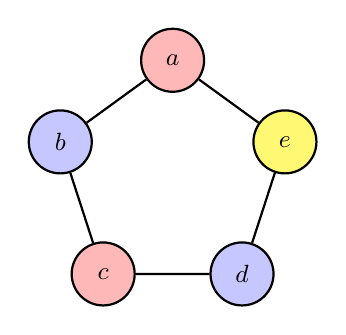
\begin{tikzpicture}
  \node[orig,c1] (a) at (90:1.5){$a$};
  \node[orig,c2] (b) at (162:1.5){$b$};
  \node[orig,c1] (c) at (234:1.5){$c$};
  \node[orig,c2] (d) at (306:1.5){$d$};
  \node[orig,c3] (e) at (18:1.5){$e$};
  \draw[thick] (a)--(b)--(c)--(d)--(e)--(a);
\end{tikzpicture}
\end{center}

% =============================================================================
\section{Carrying Example 1 onto the hardware geometry}
\label{sec:geometry}
% =============================================================================

Stages 1 finished with an \emph{abstract} graph $G'$. The machine, however, needs
\emph{points in the plane}: atoms are adjacent exactly when they sit within the
blockade radius $r$. We now finish the single-edge example (Section~2) by hand,
because there $G'$ is small enough to place directly.

Recall $G'$ was the $4$-cycle $u_1-u_2-v_2-v_1-u_1$. Its \emph{edges} are the four
sides of the cycle; its \emph{non-edges} are the two ``diagonals''
$\{u_1,v_2\}$ and $\{u_2,v_1\}$. To realize this as a unit-disk graph we place the
four atoms at the corners of a unit square in cycle order, so that each
\emph{side} (an edge of $G'$) has length $1$ and each \emph{diagonal} (a non-edge)
has length $\sqrt{2}\approx 1.41$. Choosing any radius with $1\le r<\sqrt2$, say
$r=1.2$, reproduces $G'$ exactly: sides fall inside the blockade, diagonals fall
outside.

\begin{center}
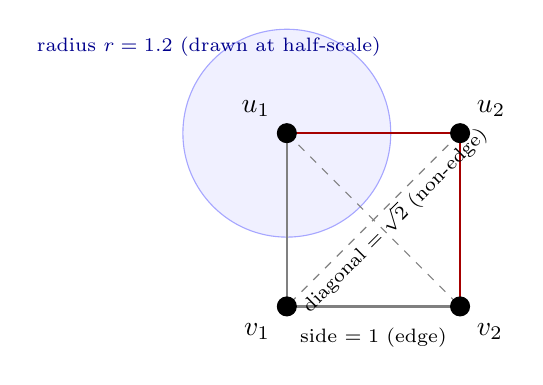
\begin{tikzpicture}[scale=2.2]
  \coordinate (u1) at (0,1);
  \coordinate (u2) at (1,1);
  \coordinate (v2) at (1,0);
  \coordinate (v1) at (0,0);
  % blockade radius illustration around u1
  \draw[blue!35,fill=blue!6] (u1) circle (0.6);
  \node[blue!55!black,font=\scriptsize] at (-0.45,1.5) {radius $r=1.2$ (drawn at half-scale)};
  % edges = square sides (within r)
  \draw[conflictedge] (u1)--(u2); % choice u1u2
  \draw[gray,thick] (v1)--(v2);   % choice v1v2
  \draw[gray,thick] (u1)--(v1);   % conflict color1
  \draw[conflictedge] (u2)--(v2); % conflict color2
  % non-edges = diagonals (outside r): draw dashed
  \draw[dashed,gray] (u1)--(v2);
  \draw[dashed,gray] (u2)--(v1);
  \node[atom,label=above left:{$u_1$}]  at (u1){};
  \node[atom,label=above right:{$u_2$}] at (u2){};
  \node[atom,label=below right:{$v_2$}] at (v2){};
  \node[atom,label=below left:{$v_1$}]  at (v1){};
  \node[font=\scriptsize] at (0.5,-0.18){side $=1$ (edge)};
  \node[font=\scriptsize,rotate=45] at (0.62,0.5){diagonal $=\sqrt2$ (non-edge)};
\end{tikzpicture}
\end{center}

\paragraph{Solve the MWIS by hand.} With all weights equal, the maximum
independent set of a $4$-cycle has size $2$: pick two atoms that are \emph{not}
joined --- a diagonal pair. Take $\{u_1,v_2\}$: they sit at distance
$\sqrt2 > r$, so they are non-adjacent and may be excited together. The
many-body ground state of the atom array settles on exactly such a pair.

\paragraph{Decode.} Read each chosen atom as ``vertex takes that color'': $u_1$
means $u\mapsto 1$, and $v_2$ means $v\mapsto 2$. This is the same proper coloring
we found abstractly --- now produced by geometry and (in the real device) by
physics. The other ground state $\{u_2,v_1\}$ decodes to the mirror coloring
$u\mapsto2, v\mapsto1$; both are correct.

\begin{tcolorbox}[colback=green!4,colframe=green!45!black,title=\textbf{What
  happens for the larger examples}]
For $P_3$, $C_4$, $C_5$, and the $k=3$ cases, the color-choice graph $G'$ is no
longer a plain $4$-cycle and usually is \emph{not} itself a unit-disk graph. Stage
2 then inserts \emph{copy} gadgets (short chains of atoms that carry an
occupation signal from one place to another) and \emph{crossing} gadgets (that let
two such signals pass without interacting), after which the whole instance is a
weighted unit-disk graph whose maximum-weight independent set still decodes to a
coloring~\cite{Pichler2018,Nguyen2023}. The bookkeeping grows, but every step is
the same kind of mechanical, exactly-reversible move shown above --- which is why
the main paper treats this stage as a once-proved, correctness-preserving black
box and spends its real effort on \emph{placing} the atoms within the device's
size and spacing limits.
\end{tcolorbox}

% =============================================================================
\section{What the five examples taught us}
% =============================================================================

\begin{table}[h]
\centering
\begin{tabular}{@{}lcccccl@{}}
\toprule
Graph & $n$ & $m$ & $k$ & $|V'|=nk$ & $\alpha(G')$ & verdict \\
\midrule
single edge $K_2$ & $2$ & $1$ & $2$ & $4$  & $2$ & $2$-colorable \\
path $P_3$        & $3$ & $2$ & $2$ & $6$  & $3$ & $2$-colorable \\
triangle $K_3$    & $3$ & $3$ & $2$ & $6$  & $2$ & \emph{not} $2$-colorable \\
triangle $K_3$    & $3$ & $3$ & $3$ & $9$  & $3$ & $3$-colorable\ $\Rightarrow\chi=3$ \\
square $C_4$      & $4$ & $4$ & $2$ & $8$  & $4$ & $2$-colorable \\
pentagon $C_5$    & $5$ & $5$ & $2$ & $10$ & $4$ & \emph{not} $2$-colorable \\
pentagon $C_5$    & $5$ & $5$ & $3$ & $15$ & $5$ & $3$-colorable\ $\Rightarrow\chi=3$ \\
\bottomrule
\end{tabular}
\caption{Every row obeys the single rule $\alpha(G')=n \iff k$-colorable. A
``not colorable'' verdict shows up cleanly as $\alpha(G')<n$.}
\end{table}

\noindent Three ideas recur:
\begin{itemize}[leftmargin=1.4em]
  \item \textbf{One slot per vertex, never two:} the choice clique caps every
        independent set at $n$, so reaching exactly $n$ is the whole game.
  \item \textbf{Conflicts live inside a single color:} two same-colored adjacent
        vertices are the \emph{only} way a one-per-vertex pick can fail, which is
        why each row carries a copy of $G$'s edges.
  \item \textbf{Too few colors $=$ pigeonhole:} $K_3$ at $k=2$ and $C_5$ at $k=2$
        fail for the same reason --- more vertices to seat than rows to seat them
        in, forcing an in-row clash. Adding a row (a color) is exactly what
        relieves the pressure.
\end{itemize}

% =============================================================================
\begin{thebibliography}{9}
\bibitem{Karp1972} R.~M.~Karp. \emph{Reducibility among combinatorial problems.}
  In \emph{Complexity of Computer Computations}, 85--103, Springer, 1972.
\bibitem{Pichler2018} H.~Pichler, S.-T.~Wang, L.~Zhou, S.~Choi, M.~D.~Lukin.
  \emph{Quantum optimization for maximum independent set using Rydberg atom
  arrays.} arXiv:1808.10816, 2018.
\bibitem{Nguyen2023} M.-T.~Nguyen, J.-G.~Liu, J.~Wurtz, M.~D.~Lukin, S.-T.~Wang,
  H.~Pichler. \emph{Quantum optimization with arbitrary connectivity using
  Rydberg atom arrays.} PRX Quantum 4, 010316, 2023.
\end{thebibliography}

\end{document}
